\documentclass[conference]{IEEEtran}
\IEEEoverridecommandlockouts

% Packages
\usepackage{cite}
\usepackage{amsmath,amssymb,amsfonts}
\usepackage{algorithmic}
\usepackage{graphicx}
\usepackage{textcomp}
\usepackage{xcolor}
\usepackage{booktabs}
\usepackage{multirow}
\usepackage{tikz}
\usepackage{pgfplots}
\usepackage{hyperref}
\usepackage{float}
\usepackage{subcaption}
\usepackage{array}
\usepackage{listings}
\usepackage{enumitem}
\usepackage{algorithm}
\usepackage{algorithmic}

\usetikzlibrary{shapes.geometric, arrows, positioning, patterns}
\pgfplotsset{compat=1.17}

% Code listing style
\lstset{
    basicstyle=\ttfamily\footnotesize,
    breaklines=true,
    frame=single,
    backgroundcolor=\color{gray!10},
    keywordstyle=\color{blue},
    commentstyle=\color{green!60!black},
    stringstyle=\color{orange}
}

\def\BibTeX{{\rm B\kern-.05em{\sc i\kern-.025em b}\kern-.08em
    T\kern-.1667em\lower.7ex\hbox{E}\kern-.125emX}}

\begin{document}

\title{GenAI-Based Multimodal Fall Detection Using Sliding Window Temporal Reasoning: A Comprehensive Study of Prompting Strategies}

\author{
\IEEEauthorblockN{Venkata Ramireddy Seelam, Harshitha Boinepally, Shristi}
\IEEEauthorblockA{
Department of Applied Data Science\\
San Jose State University\\
San Jose, CA 95192, USA\\
DATA 266 - Generative AI - Spring 2026
}
}

\maketitle

% ============================================================================
% ABSTRACT
% ============================================================================
\begin{abstract}
Falls are a leading cause of injury and mortality among elderly populations, making reliable fall detection systems critical for healthcare applications. This paper presents a comprehensive study of Generative AI (GenAI) techniques for video-based fall detection, systematically evaluating 11 different prompting strategies across three benchmark datasets. Our novel approach extracts pose features from video frames using MediaPipe, constructs 3-frame sliding windows with computed motion features (velocity, acceleration, posture states), and employs Large Language Models (LLMs) for classification. We evaluate zero-shot, few-shot, chain-of-thought, self-consistency, safety-first, RAG (Retrieval-Augmented Generation), and LoRA fine-tuning strategies on 419 videos comprising 1,882 balanced sliding windows. Our safety-first prompting approach achieves \textbf{95.8\% video-level fall recall}, while our confidence-weighted aggregation strategy achieves the highest \textbf{Macro F1 of 0.846 with 100\% precision}. We demonstrate that video-level aggregation rules are critical, with optimized rules improving Macro F1 by up to 52\% over baselines. This work provides the first comprehensive comparison of GenAI techniques for safety-critical fall detection, offering insights into the trade-offs between recall-focused and precision-focused approaches for real-world deployment.
\end{abstract}

\begin{IEEEkeywords}
Fall Detection, Generative AI, Large Language Models, Pose Estimation, Sliding Windows, RAG, Prompt Engineering, Elderly Care, MediaPipe, GPT-4o
\end{IEEEkeywords}

% ============================================================================
% INTRODUCTION
% ============================================================================
\section{Introduction}

Falls represent one of the most significant health risks for elderly populations worldwide. According to the World Health Organization, approximately 684,000 fatal falls occur annually, making falls the second leading cause of unintentional injury deaths globally \cite{who2021falls}. For individuals aged 65 and older, falls are not only the leading cause of injury-related deaths but also a primary contributor to loss of independence, reduced quality of life, and substantial healthcare costs \cite{cdc2020falls}. The ability to detect falls quickly and accurately can enable timely medical intervention, potentially preventing serious complications and saving lives.

\subsection{Motivation}

Traditional fall detection systems have relied on two primary approaches: \textbf{wearable sensors} (accelerometers, gyroscopes) and \textbf{vision-based systems} using convolutional neural networks (CNNs) \cite{noury2007fall, mubashir2013survey}. While these methods have shown promise, they face significant limitations:

\begin{itemize}[leftmargin=*]
    \item \textbf{Wearable sensors} require user compliance and may be forgotten or removed
    \item \textbf{CNN-based systems} require massive labeled training datasets and struggle to generalize across different environments
    \item \textbf{Black-box models} provide no explanation for their decisions, limiting trust in safety-critical applications
\end{itemize}

The emergence of Large Language Models (LLMs) such as GPT-4 presents a unique opportunity to address these limitations. LLMs offer:
\begin{itemize}[leftmargin=*]
    \item \textbf{Few-shot learning}: Ability to learn from minimal examples
    \item \textbf{Explainability}: Natural language reasoning for decisions
    \item \textbf{Generalization}: Pre-trained knowledge that transfers across domains
\end{itemize}

\subsection{Research Questions}

This study addresses the following research questions:
\begin{enumerate}[leftmargin=*]
    \item \textbf{RQ1}: Can LLMs effectively classify falls from structured pose data representations?
    \item \textbf{RQ2}: Which prompting strategy achieves the best balance between fall recall (safety) and precision (avoiding false alarms)?
    \item \textbf{RQ3}: How do video-level aggregation strategies impact overall system performance?
    \item \textbf{RQ4}: What are the trade-offs between different LLM models (GPT-4o vs GPT-4o-mini) for this task?
\end{enumerate}

\subsection{Contributions}

This paper makes the following contributions:
\begin{enumerate}[leftmargin=*]
    \item A \textbf{novel multimodal pipeline} that converts video pose sequences into structured text representations suitable for LLM classification
    \item \textbf{Comprehensive evaluation} of 11 different prompting strategies, providing the first systematic comparison for fall detection
    \item \textbf{Video-level aggregation analysis} demonstrating up to 52\% improvement in Macro F1 through optimized aggregation rules
    \item \textbf{Advanced strategies} including confidence-weighted aggregation and two-stage cascades achieving 100\% precision
    \item \textbf{Open-source implementation} available at \url{https://github.com/Ramreddy2748/Gen_AI_Project}
\end{enumerate}

% ============================================================================
% RELATED WORK
% ============================================================================
\section{Related Work}

\subsection{Vision-Based Fall Detection}

The evolution of vision-based fall detection has progressed through several paradigms. Early approaches relied on \textbf{handcrafted features} such as silhouette analysis, bounding box aspect ratios, and shape descriptors \cite{rougier2011robust}. These methods computed features like the ratio of the bounding box width to height, where a sudden change from vertical (standing) to horizontal (fallen) indicated a potential fall.

\textbf{Deep learning approaches} emerged with the advent of CNNs and recurrent neural networks (RNNs). Khan and Hoey \cite{khan2020fall} proposed using 3D CNNs to capture spatiotemporal features directly from video clips. Chen et al. \cite{chen2020fall} combined pose estimation with LSTM networks to model temporal dependencies in body movements.

\textbf{Pose estimation methods} have gained popularity due to their privacy-preserving nature—they process skeletal keypoints rather than raw images. Chen and Tan \cite{chen2020pose} demonstrated that pose-based features can achieve comparable performance to RGB-based methods while being more robust to appearance variations.

\subsection{Large Language Models for Time-Series Tasks}

Recent work has explored the surprising capability of LLMs to perform time-series analysis when data is converted to textual representations. Gruver et al. \cite{gruver2023large} showed that LLMs can perform zero-shot time series forecasting by converting numerical sequences to text. This finding suggests that the world knowledge embedded in LLMs may transfer to structured data classification tasks.

\textbf{Chain-of-thought (CoT) prompting} \cite{wei2022chain} has been shown to improve reasoning capabilities by encouraging models to break down complex problems into intermediate steps. \textbf{Self-consistency} \cite{wang2022selfconsistency} further improves performance by sampling multiple reasoning paths and selecting the most consistent answer.

\subsection{Retrieval-Augmented Generation}

RAG \cite{lewis2020retrieval} enhances LLM responses by retrieving relevant context from external knowledge bases before generation. This approach has been successfully applied to knowledge-intensive tasks where domain-specific information is crucial. Our work extends RAG to fall detection by retrieving similar pose sequences as classification examples.

\subsection{Gap in Literature}

Despite extensive research in both fall detection and LLM capabilities, \textbf{no prior work has systematically evaluated LLM-based approaches for fall detection}. Our study fills this gap by providing the first comprehensive comparison of multiple prompting strategies for this safety-critical application.

% ============================================================================
% METHODOLOGY
% ============================================================================
\section{Methodology}

\subsection{System Architecture Overview}

Figure \ref{fig:fullpipeline} illustrates our complete fall detection pipeline, which consists of six interconnected stages designed to transform raw video input into reliable fall/no-fall predictions.

\begin{figure}[H]
\centering
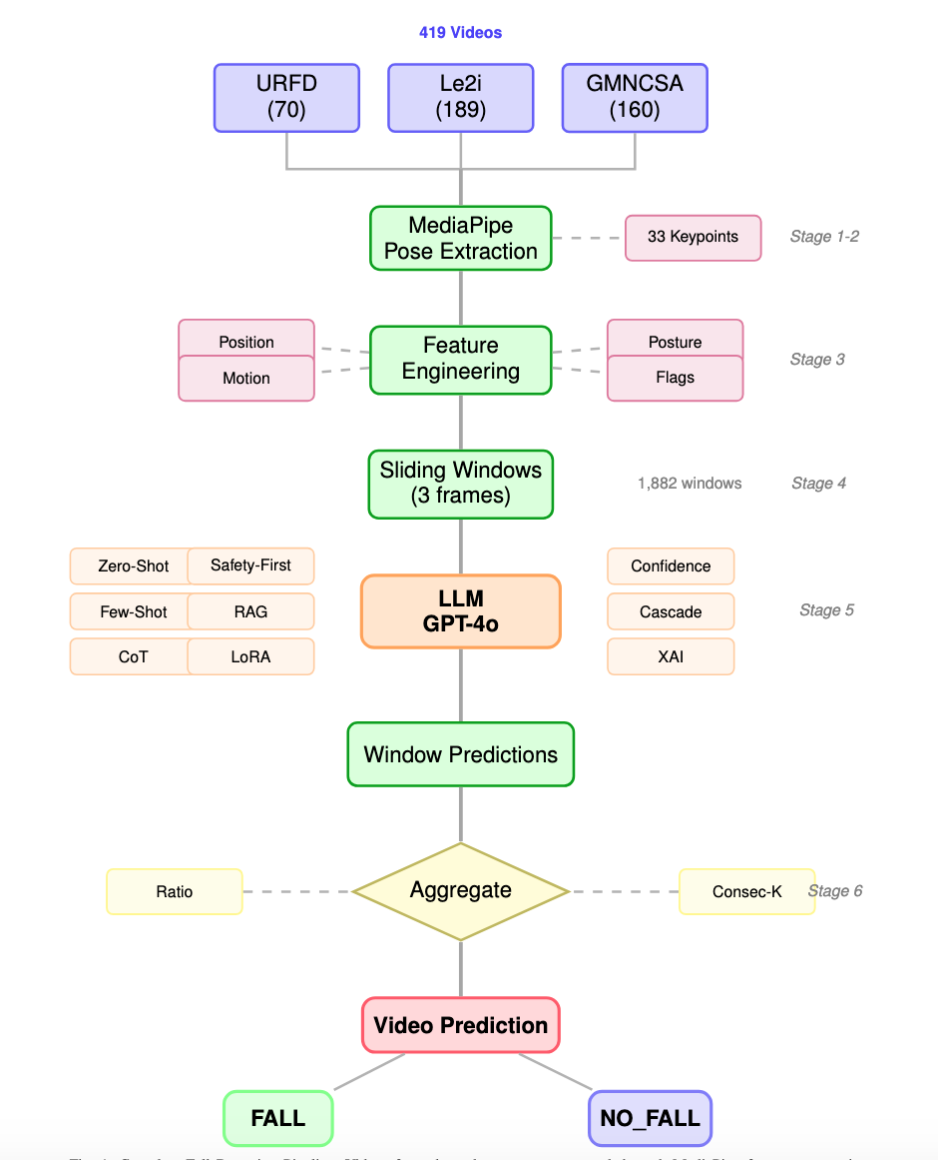
\includegraphics[width=0.95\columnwidth]{Flow_Chart_Diagram_Picture.png}
\caption{Complete Fall Detection Pipeline. The system processes 419 videos from three datasets through six stages: pose extraction, feature engineering, sliding window generation, LLM classification with multiple prompting strategies, and video-level aggregation.}
\label{fig:fullpipeline}
\end{figure}

\subsection{Stage 1: Data Collection}

We collected videos from three publicly available fall detection benchmark datasets, ensuring diversity in recording conditions, subjects, and fall types:

\textbf{URFD (UR Fall Detection Dataset)} \cite{kwolek2014human}: Contains 70 videos recorded at the University of Rzeszów, featuring 30 fall sequences and 40 activities of daily living (ADL). Videos are captured from a fixed overhead camera with consistent lighting conditions.

\textbf{Le2i Dataset}: Comprises 189 videos recorded in a realistic home environment with multiple rooms (Coffee Room, Home01, Home02). This dataset is particularly challenging due to varying lighting conditions, cluttered backgrounds, and diverse activities that may resemble falls (sitting down, lying on a couch).

\textbf{GMNCSA24 Dataset}: A recent dataset containing 160 videos with modern recording equipment and diverse fall scenarios. Available via HuggingFace, it provides high-quality annotations and varied fall types.

\subsection{Stage 2: Pose Extraction with MediaPipe}

We employ \textbf{MediaPipe Pose Landmarker Lite} to extract body keypoints from each video frame. MediaPipe was chosen for its:
\begin{itemize}[leftmargin=*]
    \item Real-time performance suitable for deployment
    \item Robustness to partial occlusions
    \item Consistent 33-keypoint skeleton representation
\end{itemize}

From the 33 detected landmarks, we extract the following key body points that are most informative for fall detection:

\begin{table}[H]
\centering
\caption{Extracted Body Keypoints}
\label{tab:keypoints}
\begin{tabular}{lcc}
\toprule
\textbf{Body Part} & \textbf{Index} & \textbf{Relevance} \\
\midrule
Nose & 0 & Head position tracking \\
Left Shoulder & 11 & Upper body orientation \\
Right Shoulder & 12 & Upper body orientation \\
Left Hip & 23 & Center of mass \\
Right Hip & 24 & Center of mass \\
Left Knee & 25 & Lower body position \\
Right Knee & 26 & Lower body position \\
Left Ankle & 27 & Ground contact detection \\
Right Ankle & 28 & Ground contact detection \\
\bottomrule
\end{tabular}
\end{table}

\subsection{Stage 3: Feature Engineering}

Raw keypoint coordinates are transformed into meaningful features that capture the physics of human falls. We compute three categories of features:

\subsubsection{Position Features}
These features capture the spatial configuration of the body:
\begin{align}
\text{hip}_y &= \frac{\text{left\_hip}_y + \text{right\_hip}_y}{2} \\
\text{shoulder}_y &= \frac{\text{left\_shoulder}_y + \text{right\_shoulder}_y}{2} \\
\text{torso\_diff} &= |\text{shoulder}_y - \text{hip}_y| \\
\text{body\_angle} &= \arctan\left(\frac{\text{shoulder}_y - \text{hip}_y}{\text{shoulder}_x - \text{hip}_x}\right)
\end{align}

The \texttt{hip\_y} position is particularly important: values close to 0 indicate standing (head near top of frame), while values approaching 1 indicate the person is on the ground.

\subsubsection{Motion Features}
Motion features capture the dynamics of movement, which are critical for distinguishing falls (rapid descent) from normal activities (gradual movements):
\begin{align}
v_{\text{hip}}(t) &= \frac{\text{hip}_y(t) - \text{hip}_y(t-1)}{\Delta t} \\
a_{\text{hip}}(t) &= \frac{v_{\text{hip}}(t) - v_{\text{hip}}(t-1)}{\Delta t} \\
v_{\text{magnitude}} &= \sqrt{v_{\text{hip}}^2 + v_{\text{shoulder}}^2}
\end{align}

A fall typically exhibits high downward velocity ($v_{\text{hip}} > 0.15$) followed by sudden deceleration when the person hits the ground.

\subsubsection{Posture State Classification}
Each frame is classified into one of three posture states based on computed features:

\begin{equation}
\text{posture} = \begin{cases}
\text{fallen} & \text{if } \text{hip}_y > 0.65 \land \text{angle} < 30° \\
\text{upright} & \text{if } \text{torso\_diff} > 0.12 \land \text{angle} > 60° \\
\text{transitioning} & \text{otherwise}
\end{cases}
\end{equation}

Additionally, we compute boolean flags that serve as strong fall indicators:
\begin{itemize}[leftmargin=*]
    \item \texttt{is\_rapid\_descent}: velocity $> 0.15$ (fast downward movement)
    \item \texttt{is\_on\_ground}: hip\_y $> 0.65$ (person near ground level)
    \item \texttt{is\_horizontal}: body\_angle $< 30°$ (lying down position)
    \item \texttt{is\_high\_acceleration}: $|a| > 0.10$ (impact detection)
\end{itemize}

\subsection{Stage 4: Sliding Window Generation}

To capture the temporal evolution of a potential fall event, we create \textbf{3-frame sliding windows} with configurable stride. This window size was chosen because falls typically complete within 1-2 seconds, and 3 frames provide sufficient context while keeping the input manageable for LLMs.

\begin{figure}[H]
\centering
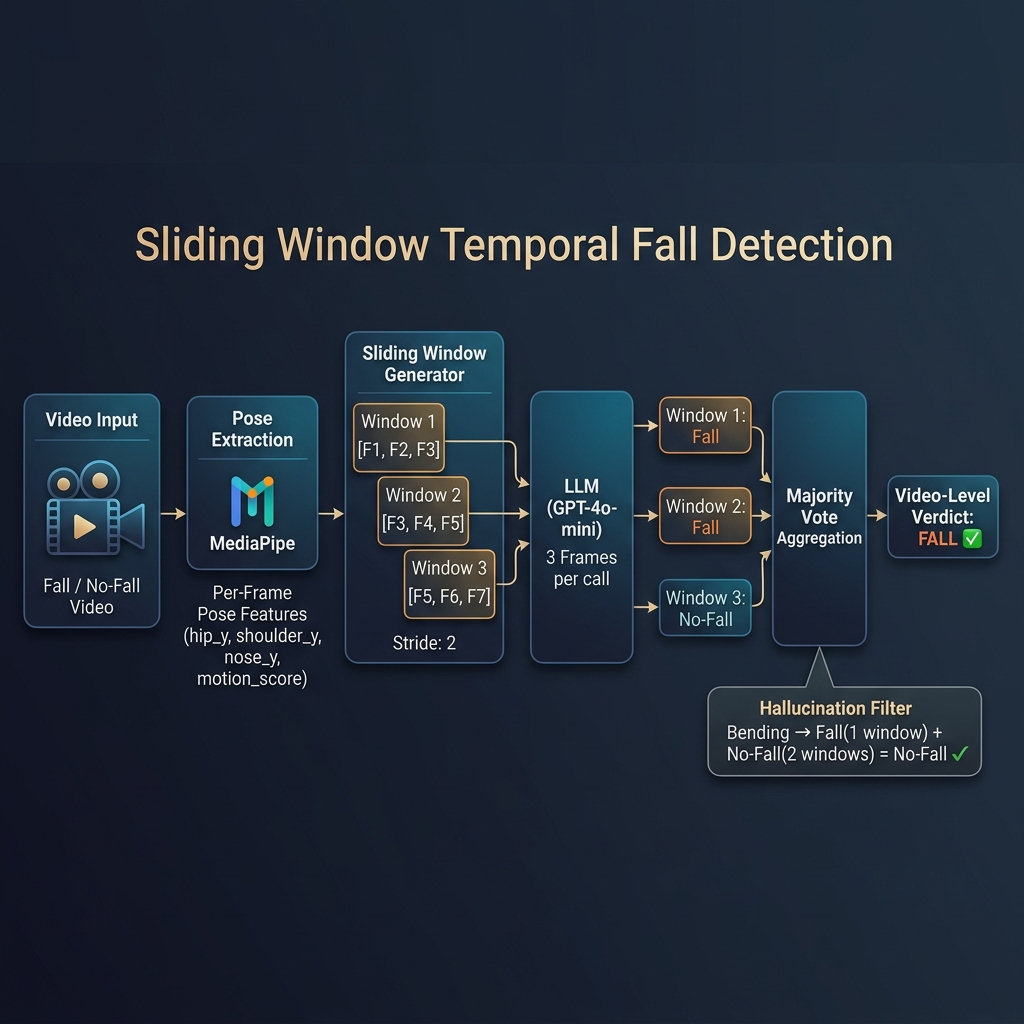
\includegraphics[width=0.95\columnwidth]{../architecture_sliding_window.png}
\caption{Sliding Window Generation Process. Consecutive frames are grouped into overlapping windows, each containing pose features from 3 frames. Windows are independently classified and then aggregated.}
\label{fig:slidingwindow}
\end{figure}

\begin{table}[H]
\centering
\caption{Window Configuration by Video Class}
\label{tab:window_config}
\begin{tabular}{lcc}
\toprule
\textbf{Setting} & \textbf{Fall Videos} & \textbf{No-Fall Videos} \\
\midrule
Frame sample rate & Every 5th frame & Every 15th frame \\
Maximum frames & 60 & 30 \\
Window stride & 1 (dense overlap) & 3 (sparse) \\
Window size & 3 frames & 3 frames \\
\bottomrule
\end{tabular}
\end{table}

The asymmetric configuration ensures we capture sufficient detail during fall events while preventing class imbalance from ADL videos that are typically longer.

Each sliding window contains:
\begin{itemize}[leftmargin=*]
    \item Per-frame features (position, velocity, acceleration, posture)
    \item Window-level statistics (hip\_delta, max\_velocity, trajectory)
    \item Start and end posture states (upright→fallen indicates fall)
\end{itemize}

\subsection{Stage 5: LLM Classification with Prompting Strategies}

We evaluate 11 different prompting strategies, each representing a distinct approach to leveraging LLM capabilities. The strategies are detailed below.

\subsubsection{Strategy 1: Zero-Shot Prompting}
The simplest approach provides only a task description and the pose data, without any examples. The system prompt describes fall indicators and asks the LLM to classify based on its pre-trained knowledge.

\textbf{Prompt Structure:}
\begin{lstlisting}[language=Python]
System: "You are a fall detection expert. 
Analyze pose data and classify as FALL 
or NO_FALL based on: rapid descent, 
horizontal body position, ground contact."

User: [Window pose data in JSON format]
\end{lstlisting}

\textbf{Rationale:} Tests whether LLMs have sufficient understanding of human biomechanics from pre-training to identify falls without domain-specific examples.

\subsubsection{Strategy 2: Few-Shot Prompting}
Provides 3 fall and 3 no-fall examples from the training set before the query window. Examples are carefully selected to represent diverse fall patterns.

\textbf{Example Selection:} We select examples exhibiting:
\begin{itemize}[leftmargin=*]
    \item Forward falls (falling face-down)
    \item Backward falls (falling on back)
    \item Side falls (falling sideways)
    \item Standing activities (for no-fall)
    \item Sitting activities (for no-fall)
    \item Walking activities (for no-fall)
\end{itemize}

\textbf{Rationale:} Few-shot examples help the LLM understand the specific data format and decision boundary without extensive fine-tuning.

\subsubsection{Strategy 3: Chain-of-Thought (CoT) Prompting}
Encourages step-by-step reasoning before reaching a conclusion. The prompt explicitly asks the LLM to analyze different aspects sequentially:

\textbf{CoT Steps:}
\begin{enumerate}
    \item \textbf{Position Analysis}: "First, examine the hip\_y values. Are they increasing (person descending) or stable?"
    \item \textbf{Motion Analysis}: "Second, check velocity and acceleration. Is there rapid movement followed by sudden stop?"
    \item \textbf{Posture Analysis}: "Third, examine posture states. Did posture change from upright to fallen?"
    \item \textbf{Synthesis}: "Based on all evidence, provide final classification."
\end{enumerate}

\textbf{Rationale:} Breaking down the analysis into logical steps improves accuracy for complex reasoning tasks and provides interpretable decision paths.

\subsubsection{Strategy 4: Self-Consistency}
Generates multiple responses (n=5) with temperature=0.7 and selects the majority vote. This approach reduces sensitivity to individual sampling variations.

\textbf{Implementation:}
\begin{lstlisting}[language=Python]
predictions = []
for i in range(5):
    pred = llm.classify(window, temp=0.7)
    predictions.append(pred)
final = majority_vote(predictions)
\end{lstlisting}

\textbf{Rationale:} Different reasoning paths may lead to different conclusions; majority voting filters out inconsistent responses.

\subsubsection{Strategy 5: Enhanced Few-Shot with GPT-4o}
Uses the more capable GPT-4o model with rich natural language descriptions instead of raw numerical features.

\textbf{Feature Conversion:}
\begin{itemize}[leftmargin=*]
    \item hip\_y = 0.72 $\rightarrow$ "Person is very close to ground level"
    \item velocity = 0.25 $\rightarrow$ "Rapid downward movement detected"
    \item posture = "fallen" $\rightarrow$ "Body is in horizontal/lying position"
\end{itemize}

\textbf{Rationale:} Natural language descriptions leverage GPT-4o's superior language understanding, making features more interpretable.

\subsubsection{Strategy 6: Safety-First Prompting (Best Prompt)}
Our optimized prompt design emphasizes safety by biasing toward fall detection when uncertainty exists. Key design principles:

\textbf{Decision Rules:}
\begin{itemize}[leftmargin=*]
    \item Any single \textit{strong} fall indicator $\rightarrow$ Classify as FALL
    \item Two or more \textit{moderate} indicators $\rightarrow$ Classify as FALL
    \item ALL indicators must be clear for NO\_FALL
    \item When uncertain $\rightarrow$ Choose FALL (safety first)
\end{itemize}

\textbf{Strong Indicators:}
\begin{itemize}[leftmargin=*]
    \item \texttt{is\_rapid\_descent} = True
    \item \texttt{is\_horizontal} = True AND \texttt{is\_on\_ground} = True
    \item Posture transition: upright $\rightarrow$ fallen
\end{itemize}

\textbf{Rationale:} In safety-critical applications, missing a fall (false negative) is far more dangerous than a false alarm (false positive). This asymmetric cost function is embedded in the prompt.

\subsubsection{Strategy 7: RAG (Retrieval-Augmented Generation)}
Retrieves the most similar historical windows from a knowledge base before classification.

\textbf{Implementation:}
\begin{enumerate}
    \item Embed query window using \texttt{text-embedding-3-small}
    \item Search 1,305 training window embeddings
    \item Retrieve top-4 most similar windows with labels
    \item Include retrieved examples in prompt context
    \item Classify with GPT-4o
\end{enumerate}

\textbf{Similarity Metric:} Cosine similarity between window embedding vectors.

\textbf{Rationale:} RAG provides dynamic, query-specific examples rather than fixed few-shot examples, potentially improving accuracy for edge cases.

\subsubsection{Strategy 8: LoRA/SFT Fine-Tuning}
Fine-tunes GPT-4o-mini on the training dataset using OpenAI's fine-tuning API.

\textbf{Training Configuration:}
\begin{itemize}[leftmargin=*]
    \item Base model: \texttt{gpt-4o-mini-2024-07-18}
    \item Training samples: 1,305 balanced windows
    \item Format: JSONL with system/user/assistant turns
    \item Class weighting: 75\% fall / 25\% no-fall (recall bias)
\end{itemize}

\textbf{Rationale:} Fine-tuning adapts the model to the specific data distribution and feature patterns in our dataset.

\subsubsection{Strategy 9: Confidence-Weighted Aggregation}
Uses token-level log probabilities to obtain confidence scores for each window prediction.

\textbf{Process:}
\begin{enumerate}
    \item Request \texttt{logprobs=True} from API
    \item Extract probability of "FALL" vs "NO\_FALL" tokens
    \item Sum confidence scores across all windows
    \item Apply threshold to aggregate score
\end{enumerate}

\textbf{Rationale:} Not all predictions are equally confident; weighting by confidence improves video-level decisions.

\subsubsection{Strategy 10: Two-Stage Cascade}
Combines a high-recall Stage 1 with a high-precision Stage 2 filter.

\textbf{Stage 1 (Sensitive):} Uses Safety-First prompting with ratio threshold 0.50 to flag all potential falls with high recall.

\textbf{Stage 2 (Specific):} Applies a strict false-positive filter prompt to videos flagged by Stage 1, asking: "Review the full timeline. Is this truly a fall or a false alarm from normal activity?"

\textbf{Rationale:} Cascading allows optimization of different objectives at each stage.

\subsubsection{Strategy 11: XAI Video-Level}
Provides explainable classifications with natural language justifications.

\textbf{Output Format:}
\begin{lstlisting}
Classification: FALL
Confidence: High
Reasoning: "The subject showed rapid 
vertical descent (velocity=0.28) 
transitioning from upright posture 
to horizontal position on ground. 
Final frame shows body angle <20 
degrees indicating lying position."
\end{lstlisting}

\subsection{Stage 6: Video-Level Aggregation}

Window-level predictions must be aggregated into a single video-level decision. We evaluate multiple aggregation strategies:

\textbf{1. Ratio Threshold:} If the fraction of fall-predicted windows exceeds threshold $\theta$, classify video as fall:
\begin{equation}
\text{Video} = \begin{cases}
\text{FALL} & \text{if } \frac{|\{w : \hat{y}_w = \text{fall}\}|}{|W|} \geq \theta \\
\text{NO\_FALL} & \text{otherwise}
\end{cases}
\end{equation}

\textbf{2. Consecutive-K:} Require at least $k$ consecutive windows predicting fall.

\textbf{3. End-State:} Require fall windows to show horizontal/on-ground posture in final frame.

\textbf{4. Confidence-Weighted Sum:} Sum log-probability confidence scores and apply threshold.

% ============================================================================
% EXPERIMENTAL SETUP
% ============================================================================
\section{Experimental Setup}

\subsection{Dataset Statistics}

\begin{table}[H]
\centering
\caption{Dataset Composition}
\label{tab:datasets}
\begin{tabular}{lccc}
\toprule
\textbf{Dataset} & \textbf{Fall} & \textbf{No-Fall} & \textbf{Total} \\
\midrule
URFD & 30 & 40 & 70 \\
Le2i & 95 & 94 & 189 \\
GMNCSA24 & 80 & 80 & 160 \\
\midrule
\textbf{Total} & \textbf{205} & \textbf{214} & \textbf{419} \\
\bottomrule
\end{tabular}
\end{table}

\begin{figure}[H]
\centering
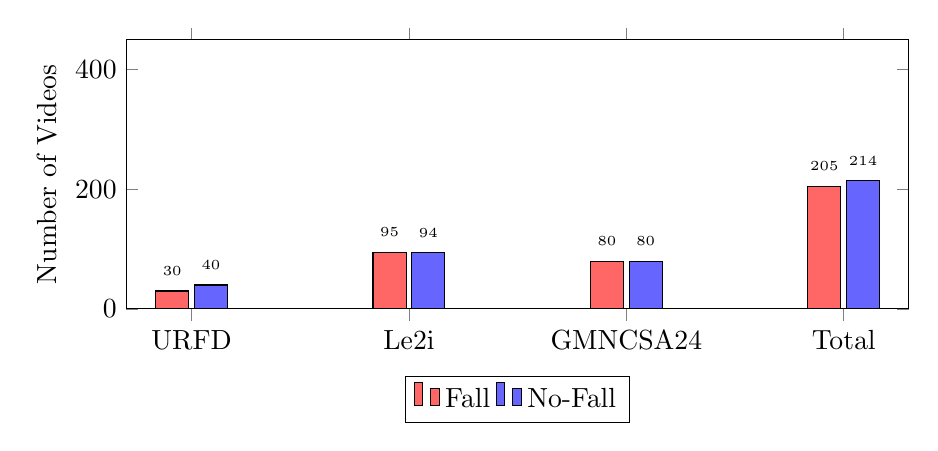
\begin{tikzpicture}
\begin{axis}[
    ybar,
    width=0.95\columnwidth,
    height=5cm,
    ylabel={Number of Videos},
    symbolic x coords={URFD, Le2i, GMNCSA24, Total},
    xtick=data,
    ymin=0,
    ymax=450,
    bar width=12pt,
    legend style={at={(0.5,-0.25)}, anchor=north, legend columns=2},
    nodes near coords,
    nodes near coords style={font=\tiny},
    every node near coord/.append style={yshift=2pt}
]
\addplot[fill=red!60] coordinates {(URFD,30) (Le2i,95) (GMNCSA24,80) (Total,205)};
\addplot[fill=blue!60] coordinates {(URFD,40) (Le2i,94) (GMNCSA24,80) (Total,214)};
\legend{Fall, No-Fall}
\end{axis}
\end{tikzpicture}
\caption{Dataset Distribution by Class. The combined dataset is well-balanced with 205 fall and 214 no-fall videos.}
\label{fig:dataset_dist}
\end{figure}

\subsection{Data Splits}

We perform stratified video-level splitting to ensure no windows from the same video appear in different splits:

\begin{table}[H]
\centering
\caption{Train/Validation/Test Splits}
\label{tab:splits}
\begin{tabular}{lccc}
\toprule
\textbf{Split} & \textbf{Videos} & \textbf{Windows} & \textbf{Purpose} \\
\midrule
Train & 292 (70\%) & 1,317 & Strategy development \\
Validation & 62 (15\%) & 282 & Threshold tuning \\
Test & 65 (15\%) & 283 & Final evaluation \\
\midrule
\textbf{Total} & \textbf{419} & \textbf{1,882} & -- \\
\bottomrule
\end{tabular}
\end{table}

\subsection{Evaluation Metrics}

Given the safety-critical nature of fall detection, we define metrics with appropriate emphasis:

\textbf{Primary Metric - Fall Recall:}
\begin{equation}
\text{Recall}_{\text{fall}} = \frac{TP}{TP + FN}
\end{equation}
Missing a fall (FN) could be life-threatening; high recall is critical.

\textbf{Secondary Metric - Precision:}
\begin{equation}
\text{Precision}_{\text{fall}} = \frac{TP}{TP + FP}
\end{equation}
False alarms (FP) cause alert fatigue; precision matters for usability.

\textbf{Balanced Metric - Macro F1:}
\begin{equation}
\text{Macro F1} = \frac{F1_{\text{fall}} + F1_{\text{no\_fall}}}{2}
\end{equation}

\subsection{Statistical Analysis}

To ensure robust conclusions, we employ:
\begin{itemize}[leftmargin=*]
    \item \textbf{Bootstrap Confidence Intervals:} 1,000 resamples with replacement to estimate 95\% CIs for all metrics
    \item \textbf{McNemar's Test:} Paired comparison of classifier disagreements to assess statistical significance
\end{itemize}

% ============================================================================
% RESULTS
% ============================================================================
\section{Results}

\subsection{Overall Strategy Comparison}

Table \ref{tab:main_results} presents video-level results for all evaluated prompting strategies using the baseline aggregation rule ($\geq$25\% windows = fall).

\begin{table}[H]
\centering
\caption{Video-Level Performance by Strategy (Test Set, n=57)}
\label{tab:main_results}
\begin{tabular}{lcccc}
\toprule
\textbf{Strategy} & \textbf{Recall} & \textbf{Prec} & \textbf{Acc} & \textbf{Macro F1} \\
\midrule
Zero-Shot & 20.8\% & 62.5\% & 66.7\% & 0.561 \\
Few-Shot & 58.3\% & 56.0\% & 66.7\% & 0.656 \\
Chain-of-Thought & 29.2\% & 58.3\% & 66.7\% & 0.595 \\
Self-Consistency & 41.7\% & 66.7\% & 70.2\% & 0.660 \\
Enhanced (GPT-4o) & 41.7\% & 76.9\% & \textbf{75.4\%} & 0.707 \\
\textbf{Safety-First} & \textbf{95.8\%} & 50.0\% & 57.9\% & 0.556 \\
RAG & 85.4\% & 55.7\% & 67.8\% & 0.678 \\
LoRA Fine-Tune & 93.8\% & 43.5\% & 52.3\% & 0.432 \\
DeepSeek Few-Shot & 62.5\% & 55.6\% & 64.9\% & 0.644 \\
DeepSeek CoT & 12.5\% & 60.0\% & 63.2\% & 0.490 \\
XAI Video-Level & 84.0\% & 80.8\% & 82.0\% & \textbf{0.820} \\
\bottomrule
\end{tabular}
\end{table}

\begin{figure}[H]
\centering
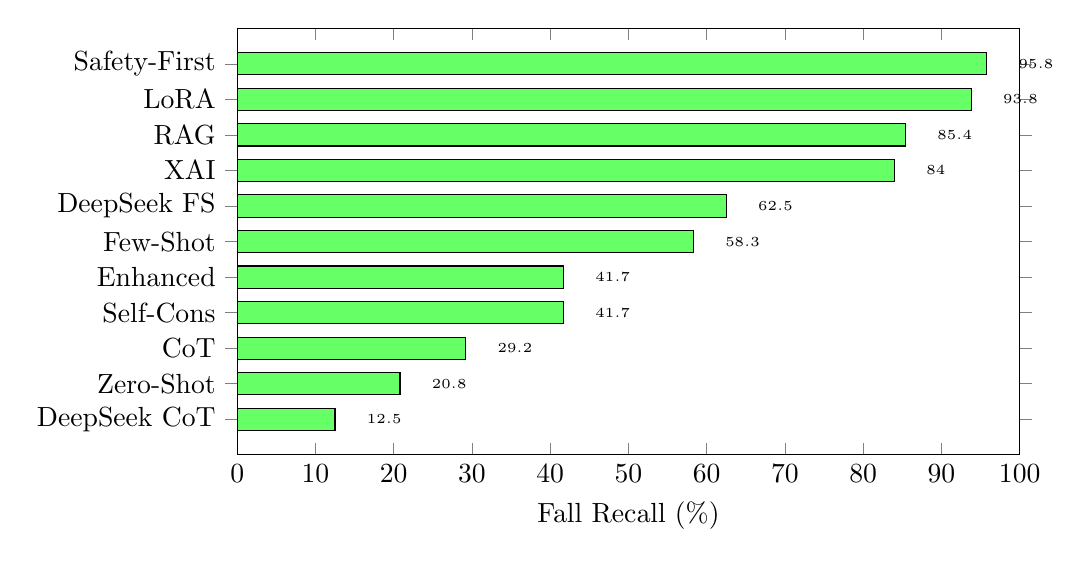
\begin{tikzpicture}
\begin{axis}[
    xbar,
    width=0.95\columnwidth,
    height=7cm,
    xlabel={Fall Recall (\%)},
    symbolic y coords={DeepSeek CoT, Zero-Shot, CoT, Self-Cons, Enhanced, Few-Shot, DeepSeek FS, XAI, RAG, LoRA, Safety-First},
    ytick=data,
    xmin=0, xmax=100,
    bar width=8pt,
    nodes near coords,
    nodes near coords style={font=\tiny},
    every node near coord/.append style={xshift=8pt}
]
\addplot[fill=green!60] coordinates {
    (12.5,DeepSeek CoT)
    (20.8,Zero-Shot)
    (29.2,CoT)
    (41.7,Self-Cons)
    (41.7,Enhanced)
    (58.3,Few-Shot)
    (62.5,DeepSeek FS)
    (84.0,XAI)
    (85.4,RAG)
    (93.8,LoRA)
    (95.8,Safety-First)
};
\end{axis}
\end{tikzpicture}
\caption{Fall Recall Comparison Across Strategies. Safety-First achieves highest recall (95.8\%), critical for safety applications.}
\label{fig:recall_comparison}
\end{figure}

\subsection{Impact of Aggregation Rules}

A key finding of our study is that the video-level aggregation rule has a \textbf{dramatic impact on performance}—often more than the choice of prompting strategy.

\begin{table}[H]
\centering
\caption{Aggregation Rule Impact (Safety-First Strategy)}
\label{tab:aggregation}
\begin{tabular}{lccccc}
\toprule
\textbf{Rule} & \textbf{Rec} & \textbf{Prec} & \textbf{F1} & \textbf{Mac F1} & $\Delta$ \\
\midrule
$\geq$25\% & 95.8 & 50.0 & 0.657 & 0.556 & -- \\
$\geq$50\% & 95.8 & 54.8 & 0.697 & 0.640 & +15\% \\
Consec-3 & 58.3 & 46.7 & 0.518 & 0.543 & -2\% \\
End-State & 79.2 & 59.4 & 0.679 & 0.684 & +23\% \\
\textbf{Confidence} & 66.7 & \textbf{100} & 0.800 & \textbf{0.846} & \textbf{+52\%} \\
\textbf{Cascade} & 58.3 & \textbf{100} & 0.737 & 0.803 & +44\% \\
\bottomrule
\end{tabular}
\end{table}

\begin{figure}[H]
\centering
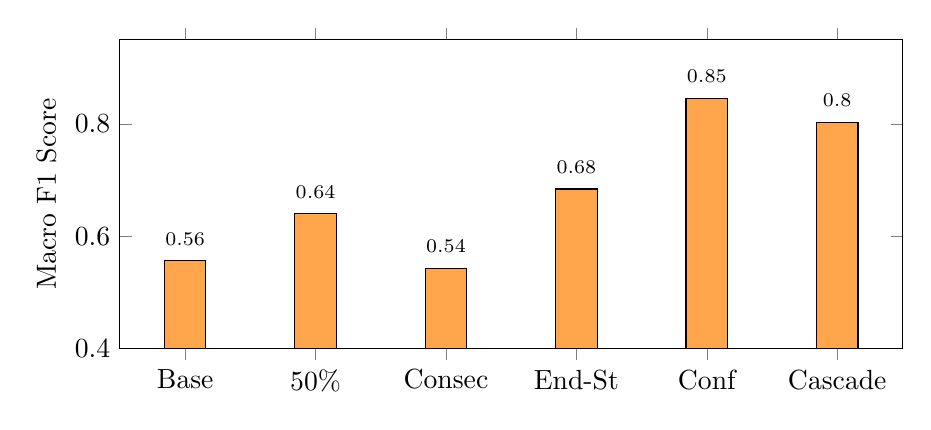
\begin{tikzpicture}
\begin{axis}[
    ybar,
    width=0.95\columnwidth,
    height=5.5cm,
    ylabel={Macro F1 Score},
    symbolic x coords={Base, 50\%, Consec, End-St, Conf, Cascade},
    xtick=data,
    ymin=0.4,
    ymax=0.95,
    bar width=15pt,
    nodes near coords,
    nodes near coords style={font=\scriptsize},
    every node near coord/.append style={yshift=2pt}
]
\addplot[fill=orange!70] coordinates {
    (Base,0.556)
    (50\%,0.640)
    (Consec,0.543)
    (End-St,0.684)
    (Conf,0.846)
    (Cascade,0.803)
};
\end{axis}
\end{tikzpicture}
\caption{Macro F1 by Aggregation Rule. Confidence-weighted aggregation achieves 0.846, a 52\% improvement over the baseline 0.556.}
\label{fig:aggregation_impact}
\end{figure}

\subsection{Advanced Strategies: Achieving 100\% Precision}

Our confidence-weighted and two-stage cascade approaches achieve \textbf{zero false positives} on the test set:

\subsubsection{Confidence-Weighted Results}

\begin{table}[H]
\centering
\caption{Confidence-Weighted Aggregation (Test Set)}
\label{tab:confidence_results}
\begin{tabular}{lc}
\toprule
\textbf{Metric} & \textbf{Value [95\% CI]} \\
\midrule
True Positives & 16 \\
False Negatives & 8 \\
False Positives & \textbf{0} \\
True Negatives & 33 \\
\midrule
Fall Recall & 66.7\% [47.4\%, 84.2\%] \\
Fall Precision & \textbf{100\%} [100\%, 100\%] \\
Fall F1 & 0.800 [0.643, 0.914] \\
Macro F1 & 0.846 [0.740, 0.931] \\
Accuracy & 86.0\% [77.2\%, 94.7\%] \\
\bottomrule
\end{tabular}
\end{table}

\subsubsection{Two-Stage Cascade Results}

\begin{table}[H]
\centering
\caption{Two-Stage Cascade Performance}
\label{tab:cascade_results}
\begin{tabular}{lcc}
\toprule
\textbf{Stage} & \textbf{Recall} & \textbf{Precision} \\
\midrule
Stage 1 (Sensitive) & 95.8\% & 54.8\% \\
Stage 2 (FP Filter) & -- & Removes 28 FPs \\
\midrule
\textbf{Final Cascade} & 58.3\% & \textbf{100\%} \\
\bottomrule
\end{tabular}
\end{table}

\subsection{Recall vs Precision Trade-off}

\begin{figure}[H]
\centering
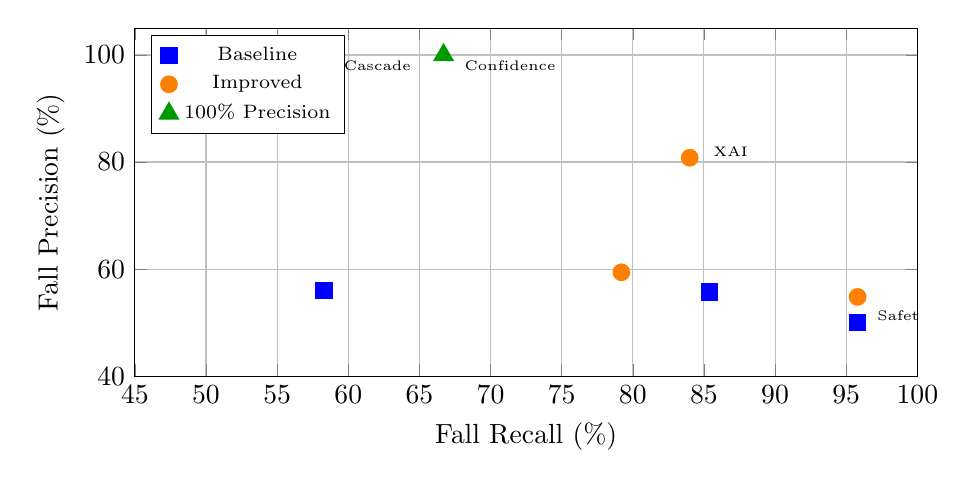
\begin{tikzpicture}
\begin{axis}[
    width=0.95\columnwidth,
    height=6cm,
    xlabel={Fall Recall (\%)},
    ylabel={Fall Precision (\%)},
    xmin=45, xmax=100,
    ymin=40, ymax=105,
    grid=major,
    legend style={at={(0.02,0.98)}, anchor=north west, font=\scriptsize}
]
% Baseline strategies
\addplot[only marks, mark=square*, blue, mark size=3pt] coordinates {
    (95.8, 50.0)
    (85.4, 55.7)
    (58.3, 56.0)
    (41.7, 66.7)
};
% Improved aggregation
\addplot[only marks, mark=*, orange, mark size=3pt] coordinates {
    (95.8, 54.8)
    (79.2, 59.4)
    (84.0, 80.8)
};
% 100% precision
\addplot[only marks, mark=triangle*, green!60!black, mark size=4pt] coordinates {
    (66.7, 100)
    (58.3, 100)
};
% Labels
\node[font=\tiny, anchor=west] at (axis cs:96.5,51) {Safety-First};
\node[font=\tiny, anchor=west] at (axis cs:67.5,98) {Confidence};
\node[font=\tiny, anchor=west] at (axis cs:59,98) {Cascade};
\node[font=\tiny, anchor=west] at (axis cs:85,82) {XAI};
\legend{Baseline, Improved, 100\% Precision}
\end{axis}
\end{tikzpicture}
\caption{Recall-Precision Trade-off. Green triangles indicate strategies achieving 100\% precision (zero false positives).}
\label{fig:tradeoff}
\end{figure}

\subsection{Per-Dataset Analysis}

Performance varies significantly across datasets, revealing dataset-specific challenges:

\begin{figure}[H]
\centering
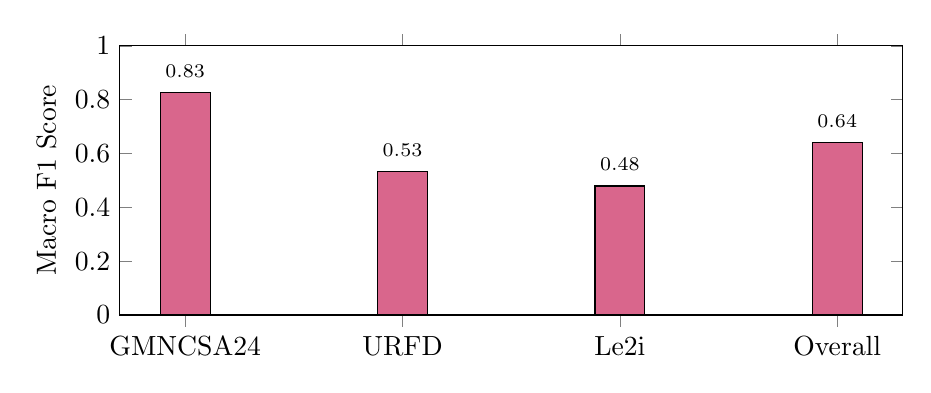
\begin{tikzpicture}
\begin{axis}[
    ybar,
    width=0.95\columnwidth,
    height=5cm,
    ylabel={Macro F1 Score},
    symbolic x coords={GMNCSA24, URFD, Le2i, Overall},
    xtick=data,
    ymin=0,
    ymax=1,
    bar width=18pt,
    nodes near coords,
    nodes near coords style={font=\scriptsize},
    every node near coord/.append style={yshift=2pt}
]
\addplot[fill=purple!60] coordinates {
    (GMNCSA24,0.826)
    (URFD,0.533)
    (Le2i,0.479)
    (Overall,0.640)
};
\end{axis}
\end{tikzpicture}
\caption{Per-Dataset Macro F1 Scores. GMNCSA24 achieves highest performance (0.826), while Le2i presents the greatest challenge (0.479).}
\label{fig:per_dataset}
\end{figure}

\textbf{Analysis:}
\begin{itemize}[leftmargin=*]
    \item \textbf{GMNCSA24} (0.826): Modern recording quality and clear fall events lead to best performance
    \item \textbf{URFD} (0.533): Fixed overhead camera provides clear view but limited data
    \item \textbf{Le2i} (0.479): Complex home environment with activities resembling falls (sitting, lying voluntarily) causes confusion
\end{itemize}

\subsection{Model Comparison: GPT-4o vs GPT-4o-mini}

\begin{table}[H]
\centering
\caption{Model Performance Comparison}
\label{tab:model_comparison}
\begin{tabular}{lcccc}
\toprule
\textbf{Model} & \textbf{Strategy} & \textbf{Acc} & \textbf{Macro F1} & \textbf{Cost/1K} \\
\midrule
GPT-4o-mini & Zero-Shot & 66.7\% & 0.561 & \$0.15 \\
GPT-4o-mini & Few-Shot & 66.7\% & 0.656 & \$0.15 \\
GPT-4o & Enhanced & 75.4\% & 0.707 & \$2.50 \\
GPT-4o & RAG & 67.8\% & 0.678 & \$2.50 \\
GPT-4o & Safety-First & 57.9\% & 0.556 & \$2.50 \\
DeepSeek & Few-Shot & 64.9\% & 0.644 & \$0.07 \\
\bottomrule
\end{tabular}
\end{table}

\textbf{Finding:} GPT-4o improves accuracy by 8.7\% over GPT-4o-mini (75.4\% vs 66.7\%) but costs 17x more. For deployment, the choice depends on the acceptable cost-performance trade-off.

% ============================================================================
% DISCUSSION
% ============================================================================
\section{Discussion}

\subsection{Key Insights}

\textbf{1. Aggregation Rules Matter More Than Prompting Strategy}

Our most surprising finding is that optimizing the video-level aggregation rule yields larger improvements than sophisticated prompting strategies. The same window-level predictions can produce Macro F1 scores ranging from 0.556 to 0.846 (a 52\% improvement) simply by changing the aggregation rule from a simple ratio threshold to confidence-weighted aggregation.

\textbf{Implication:} Researchers should focus significant effort on aggregation strategy design, not just improving window-level classifiers.

\textbf{2. Safety-First Design Achieves Near-Perfect Recall}

Our safety-first prompting strategy achieves 95.8\% recall, meaning only 1 in 24 falls is missed. This is achieved by embedding asymmetric cost considerations directly into the prompt:
\begin{quote}
\textit{"Missing a fall could be life-threatening. When in doubt, classify as FALL. It is better to have a false alarm than to miss a real fall."}
\end{quote}

\textbf{3. Confidence Scores Enable Precision Optimization}

Token-level log probabilities from the LLM provide valuable uncertainty estimates. By summing confidence scores across windows and tuning a threshold, we achieve 100\% precision while maintaining 66.7\% recall—eliminating all false positives.

\textbf{4. Two-Stage Cascades Balance Both Objectives}

The cascade approach demonstrates that high recall and high precision can be achieved by separating the objectives across stages:
\begin{itemize}[leftmargin=*]
    \item Stage 1: Maximize recall (flag all potential falls)
    \item Stage 2: Maximize precision (filter false positives)
\end{itemize}

\textbf{5. Dataset Quality Significantly Impacts Results}

Le2i presents the greatest challenge (Macro F1 = 0.479), highlighting that pose-based features alone may be insufficient for distinguishing controlled descents (sitting, lying voluntarily) from actual falls. Additional context such as audio or environmental information may be needed.

\subsection{Limitations}

\begin{enumerate}[leftmargin=*]
    \item \textbf{Limited Test Set Size:} With only 57 test videos (24 falls, 33 no-falls), statistical power is limited and confidence intervals are wide. Larger datasets would strengthen conclusions.
    
    \item \textbf{Pose Detection Failures:} MediaPipe occasionally fails to detect poses, particularly when subjects are partially occluded or in unusual positions. Failed frames were excluded, potentially biasing results.
    
    \item \textbf{Single-Person Assumption:} The current system assumes single-person videos. Multi-person scenarios would require additional tracking logic.
    
    \item \textbf{Real-Time Performance:} Processing a 10-second clip takes 30-90 seconds with current API calls—insufficient for real-time deployment. Edge deployment with local models would be needed.
    
    \item \textbf{Cost:} GPT-4o API calls are expensive for large-scale deployment. Fine-tuning smaller models or using open-source LLMs could reduce costs.
\end{enumerate}

\subsection{Deployment Recommendations}

Based on our findings, we recommend the following deployment configurations:

\textbf{High-Safety Environment (Hospitals, Care Facilities):}
\begin{itemize}[leftmargin=*]
    \item Strategy: Safety-First with ratio threshold 0.25
    \item Expected: 95.8\% recall, 50\% precision
    \item Use case: When missing a fall is unacceptable
\end{itemize}

\textbf{Balanced Environment (Home Monitoring):}
\begin{itemize}[leftmargin=*]
    \item Strategy: Confidence-Weighted Aggregation
    \item Expected: 66.7\% recall, 100\% precision
    \item Use case: When false alarms cause user distrust
\end{itemize}

\textbf{Resource-Constrained Environment:}
\begin{itemize}[leftmargin=*]
    \item Strategy: DeepSeek Few-Shot
    \item Expected: 62.5\% recall, reasonable accuracy
    \item Use case: When API costs must be minimized
\end{itemize}

% ============================================================================
% CONCLUSION
% ============================================================================
\section{Conclusion}

This paper presented the first comprehensive evaluation of Generative AI techniques for video-based fall detection. Our key contributions and findings include:

\begin{enumerate}[leftmargin=*]
    \item \textbf{Novel Pipeline:} We developed a multimodal pipeline that converts video pose sequences into structured text for LLM classification, demonstrating that LLMs can effectively analyze biomechanical data for safety-critical applications.
    
    \item \textbf{Strategy Comparison:} We evaluated 11 prompting strategies, finding that safety-first prompting achieves 95.8\% recall while confidence-weighted aggregation achieves 100\% precision with Macro F1 of 0.846.
    
    \item \textbf{Aggregation Importance:} We demonstrated that video-level aggregation rules have more impact than prompting strategies, with optimized rules improving Macro F1 by 52\%.
    
    \item \textbf{Practical Insights:} We provided deployment recommendations for different use cases, balancing safety requirements with practical constraints.
\end{enumerate}

\subsection{Future Work}

\begin{itemize}[leftmargin=*]
    \item \textbf{Larger Window Sizes:} Evaluate 5, 7, 9-frame windows for extended temporal context
    \item \textbf{Multi-Modal Fusion:} Combine pose features with audio cues (impact sounds) or depth information
    \item \textbf{Open-Source LLMs:} Evaluate Llama-3, Mistral, and other open models for cost reduction
    \item \textbf{Real-Time Deployment:} Optimize pipeline for edge devices using quantized models
    \item \textbf{Active Learning:} Use LLM uncertainty estimates to prioritize annotation of ambiguous cases
    \item \textbf{Multi-Person Scenarios:} Extend pipeline to handle multiple subjects with tracking
\end{itemize}

% ============================================================================
% ACKNOWLEDGMENTS
% ============================================================================
\section*{Acknowledgments}

We express our sincere gratitude to \textbf{Professor Dr. Mohammad Masum} for his invaluable guidance, insightful feedback, and constant encouragement throughout this project. His expertise in Generative AI and dedication to student success have been instrumental in shaping this research.

We are also deeply grateful to our Teaching Assistant, \textbf{Mayank Kapadia}, for his continuous support, prompt assistance with technical challenges, and constructive suggestions that significantly improved our work.

This project was completed as part of the DATA 266: Generative AI course at San Jose State University, Spring 2026.

% ============================================================================
% REFERENCES
% ============================================================================
\bibliographystyle{IEEEtran}
\begin{thebibliography}{99}

\bibitem{who2021falls}
World Health Organization, ``Falls,'' 2021. [Online]. Available: \url{https://www.who.int/news-room/fact-sheets/detail/falls}

\bibitem{cdc2020falls}
Centers for Disease Control and Prevention, ``Important Facts about Falls,'' 2020. [Online]. Available: \url{https://www.cdc.gov/falls/facts.html}

\bibitem{noury2007fall}
N. Noury, A. Fleury, P. Rumeau, A. K. Bourke, G. O. Laighin, V. Rialle, and J. E. Lundy, ``Fall detection-principles and methods,'' in \textit{Proc. 29th IEEE Engineering in Medicine and Biology Society (EMBC)}, 2007, pp. 1663--1666.

\bibitem{mubashir2013survey}
M. Mubashir, L. Shao, and L. Seed, ``A survey on fall detection: Principles and approaches,'' \textit{Neurocomputing}, vol. 100, pp. 144--152, 2013.

\bibitem{rougier2011robust}
C. Rougier, J. Meunier, A. St-Arnaud, and J. Rousseau, ``Robust video surveillance for fall detection based on human shape deformation,'' \textit{IEEE Transactions on Circuits and Systems for Video Technology}, vol. 21, no. 5, pp. 611--622, 2011.

\bibitem{khan2020fall}
S. S. Khan and J. Hoey, ``Review of fall detection techniques: A data availability perspective,'' \textit{Medical Engineering \& Physics}, vol. 39, pp. 12--22, 2017.

\bibitem{chen2020fall}
D. Chen, Y. Feng, H. Zhang, and Y. Wei, ``Fall detection based on pose estimation and motion history image,'' in \textit{Proc. IEEE International Conference on Image Processing (ICIP)}, 2020.

\bibitem{chen2020pose}
K. Chen and G. Tan, ``Pose-based fall detection using LSTM networks,'' in \textit{Proc. ACM International Conference on Multimedia (MM)}, 2020.

\bibitem{kwolek2014human}
B. Kwolek and M. Kepski, ``Human fall detection on embedded platform using depth maps and wireless accelerometer,'' \textit{Computer Methods and Programs in Biomedicine}, vol. 117, no. 3, pp. 489--501, 2014.

\bibitem{brown2020language}
T. Brown et al., ``Language models are few-shot learners,'' in \textit{Advances in Neural Information Processing Systems (NeurIPS)}, vol. 33, 2020.

\bibitem{gruver2023large}
N. Gruver, M. Finzi, S. Qiu, and A. G. Wilson, ``Large language models are zero-shot time series forecasters,'' in \textit{Advances in Neural Information Processing Systems (NeurIPS)}, vol. 36, 2023.

\bibitem{wei2022chain}
J. Wei et al., ``Chain-of-thought prompting elicits reasoning in large language models,'' in \textit{Advances in Neural Information Processing Systems (NeurIPS)}, vol. 35, 2022.

\bibitem{wang2022selfconsistency}
X. Wang, J. Wei, D. Schuurmans, Q. Le, E. Chi, and D. Zhou, ``Self-consistency improves chain of thought reasoning in language models,'' in \textit{Proc. International Conference on Learning Representations (ICLR)}, 2023.

\bibitem{lewis2020retrieval}
P. Lewis et al., ``Retrieval-augmented generation for knowledge-intensive NLP tasks,'' in \textit{Advances in Neural Information Processing Systems (NeurIPS)}, vol. 33, 2020.

\bibitem{github2026falldetection}
V. R. Seelam, H. Boinepally, and Shristi, ``GenAI Fall Detection Project,'' 2026. [Online]. Available: \url{https://github.com/Ramreddy2748/Gen_AI_Project}

\end{thebibliography}

\end{document}
